\documentclass[tikz]{standalone}
\usepackage{tikz}
\usetikzlibrary{arrows.meta,fit,backgrounds,positioning}

\begin{document}
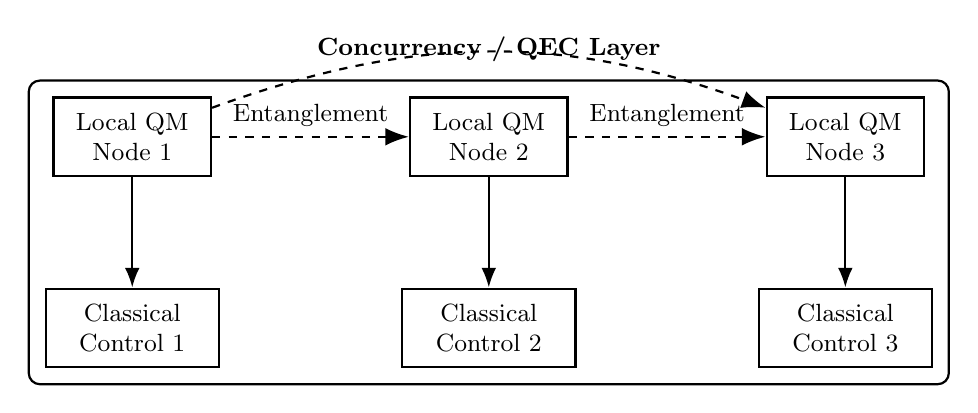
\begin{tikzpicture}[font=\small, node distance=2.5cm]

% Styles
\tikzset{
  qmem/.style={
    draw,
    thick,
    rectangle,
    minimum width=2cm,
    minimum height=1cm,
    align=center
  },
  classical/.style={
    draw,
    thick,
    rectangle,
    minimum width=2.2cm,
    minimum height=1cm,
    align=center
  },
  entangle/.style={
    dashed,
    -{Latex[length=3mm]},
    line width=0.8pt
  },
  control/.style={
    -{Latex[length=2.5mm]},
    line width=0.8pt
  }
}

% Nodes (Local Quantum Memories)
\node[qmem] (lqm1) {Local QM\\Node 1};
\node[qmem, right=of lqm1] (lqm2) {Local QM\\Node 2};
\node[qmem, right=of lqm2] (lqm3) {Local QM\\Node 3};

% Classical control nodes
\node[classical, below=1.4cm of lqm1] (cc1) {Classical\\Control 1};
\node[classical, below=1.4cm of lqm2] (cc2) {Classical\\Control 2};
\node[classical, below=1.4cm of lqm3] (cc3) {Classical\\Control 3};

% Entanglement channels (dashed lines)
\draw[entangle] (lqm1) -- (lqm2) node[midway, above] {Entanglement};
\draw[entangle] (lqm2) -- (lqm3) node[midway, above] {Entanglement};
\draw[entangle] (lqm1) to[out=20, in=160] (lqm3);

% Control links
\draw[control] (lqm1) -- (cc1);
\draw[control] (lqm2) -- (cc2);
\draw[control] (lqm3) -- (cc3);

% Overarching concurrency/QEC layer box
\begin{scope}[on background layer]
\node[draw, thick, rounded corners,
      fit=(lqm1)(lqm2)(lqm3)(cc1)(cc2)(cc3),
      label={[yshift=0.1cm]above:\textbf{Concurrency / QEC Layer}},
      inner sep=0.2cm] {};
\end{scope}

\end{tikzpicture}
\end{document}
